%!TEX root = ../main.tex
%%%%%%%%%%%%%%%%%%%%%%%%%%%%%%%%%%
% Links:
%
% Difficulty:
% Companies: 
%%%%%%%%%%%%%%%%%%%%%%%%%%%%%%%%%%


%\begin{figure}
%   \centering
%   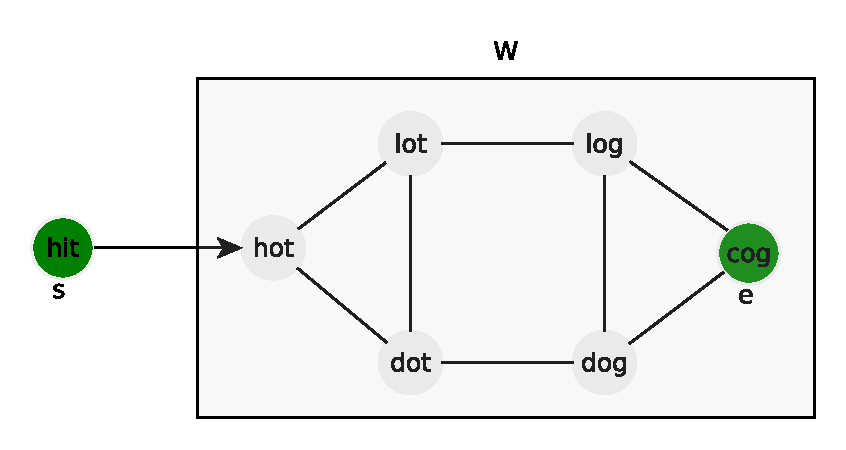
\includegraphics[width=\textwidth]{sources/word_ladder/images/example1}
%   \caption[Sample short cpation]{Sample Caption}.
%   \label{fig:word_ladder:example1}
%\end{figure}

\chapter{Word Ladder}
\label{ch:word_ladder}
\section*{Introduction}
\begin{wrapfigure}{r}{0.1\textwidth}
    \vspace{-30pt}
    \begin{center}
        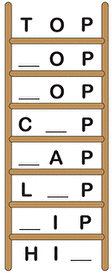
\includegraphics[scale=0.5]{sources/word_ladder/images/top-word-ladder}
    \end{center}
  \end{wrapfigure}
String is a popular topic in coding interviews and there are literally countless examples of real-world interviews where strings are involved in some way or another.
This manuscript already contains several string questions in chapters: \ref{ch:string_to_int} (page \pageref{ch:string_to_int}), \ref{ch:string_reverse} (page \pageref{ch:string_reverse}) and \ref{ch:two_string_anagram} (page \pageref{ch:two_string_anagram})).
Among this plethora of questions, \textit{word ladder} is definitely one of the most known and feared (at the time of writing it has one of the lowest acceptance rates on \href{https://leetcode.com/problems/word-ladder/}{leetcode.com}), as is considered a quite challenging and hard problem to solve during a live coding interview. 
We feel however that its bad reputation is unjustified because, as we will see below, it can be approached by using known algorithmic tools and concepts when framed as a graph connectivity problem.


\section{Problem statement}
\begin{exercise}
\label{example:word_ladder:exercice1}
We are given two strings $s$ and $e$ and a list of strings $W=\{w_0, w_1,\ldots,w_{n-1}\}$ of size $n$.
Let a sequence $S=s_0 = s \rightarrow s_1 \rightarrow s_2 \rightarrow \ldots \rightarrow s_n = e$ be defined as a \textit{transformation} if and only if:
\begin{itemize}
    \item $s_i$ differs from from its adjecent neighboring strings in the sequence, $s_{i-1}$ and $s_{i+1}$, in exactly one character;
    \item each elements of the sequence, from second to last, is also in $W$ i.e. $s_i \in W \: \: 1 \leq n-1 $
\end{itemize}
Write a function that given $s,e$ and $W$ returns the length of the smallest valid transformation.
If no transformation exists the function should return $0$.

    %example1
    \begin{example}
        \label{example:word_ladder:example1}
        \hfill \\
        Given $s=$\textit{hit},  $e=$\textit{cog} and $W=\{$\textit{hot},\textit{dot},\textit{dog},\textit{lot},\textit{log},\textit{cog}$\}$, the function returns $5$.
        A possible valid transformation  of minimal length is: \textit{hit} $\rightarrow$ \textit{hot} $\rightarrow$ \textit{dot} $\rightarrow$ \textit{dog} $\rightarrow$ \textit{cog}.

        Notice that if for instance $e=$\textit{fog}, the the function would return $0$ as \textit{fog} $\notin W$.
    \end{example}

\end{exercise}

\section{Clarification Questions}

\begin{QandA}
    \item What is the maximum length of each word in $W$?
    \begin{answered}
        \textit{Up to $10$ characters.}
    \end{answered}
    
    \item Is it guaranteed for all input strings ($s$ and $e$ included) to be of the same length?
    \begin{answered}
        \textit{Yes}
    \end{answered}

    \item Are there duplicates in $W$?
    \begin{answered}
        \textit{No, you might assume $W$ to only contains unique words.}
    \end{answered}

    \item How many words are in $W$ at most?
    \begin{answered}
        \textit{Up to $2\times 10^4$.}
    \end{answered}

    \item Should $s$ be in $W$?
    \begin{answered}
        \textit{No, that is not a necessary condition.}
    \end{answered}

\end{QandA}



\subsection{BFS}
\label{word_ladder:sec:bruteforce}
Let's start by noticing that if $e \notin W$ then we can immediately return zero, as the problem requires this condition to be met (see Figure \ref{fig:word_ladder:example1_impossible}).

In the other scenario where $e \in W$, the key to solving this problem effectively in a coding interview setting is to reframe it as a graph problem. 
The statement already mentions the concept of a sequence which might be a hint leading us into thinking about graph paths (and about the shortest distance between two nodes).

But how can we construct a graph out of a problem instance?
Let's imagine a graph $G=(V,E)$ where:
\begin{itemize}
    \item all the nodes in $V$ have a one-to-one mapping to the input strings in $W$ i.e. for each word $w_i$ we create a node that we label with $w_i$;
    \item there is an edge between two nodes $w_i$ and $w_j$ when they (their labels to be precise, or associated words in $W$) differ by one character.
\end{itemize}
An example of such a graph depicting Example \ref{example:word_ladder:example1} is given in Figure \ref{example:word_ladder:example1}; we can clearly see how the words in $W$ form a graph under the aforementioned rules.

Once we know we can easily construct a graph out of the problem instance, we are basically done as we can apply a \textbf{BFS} visit to $G$ starting from node $s$ and return the length of the shortest path to $e$.
Nothing fancier than a simple visit is required to solve this problem.

But is this approach going to be efficient enough? The visit is going to run in $O(|V|+|E|)$ time and $O(|V|)$ space but on top of that, we need to add the time and space required to build $G$ itself. 
Thankfully, we know right away that the answer is yes because a node will never have more than $10\times 26$ neighbors as:
\begin{itemize}
    \item the maximum length of a string in $W$ is $10$;
    \item each letter can only take values from the set of the lower-case English letters
\end{itemize}.
Therefore, the graph will never have more than $|E|=O(260|V|)=O(|V|)=O(|W|)$ edges.

An implementation of this idea is shown in Listing \ref{list:word_ladder_bfs}

    \begin{figure}[]
        \centering
        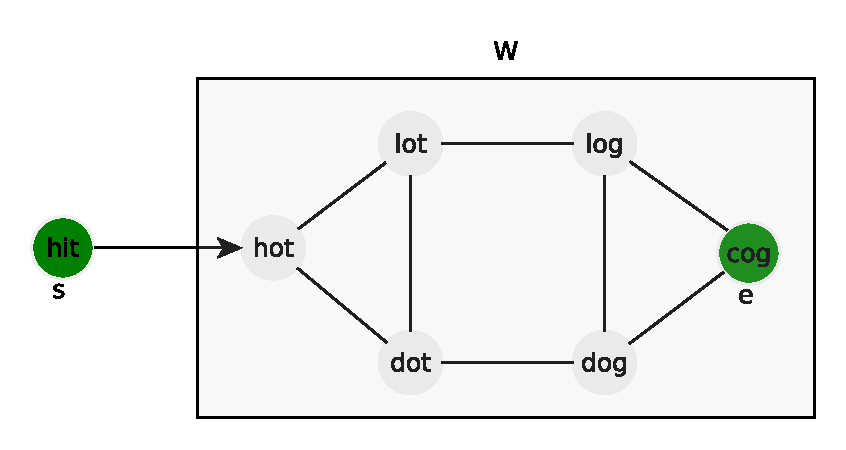
\includegraphics[width=\textwidth]{sources/word_ladder/images/example1}
        \caption[n]{Graph representation of Example \ref{example:word_ladder:example1}.}
        \label{fig:word_ladder:example1}
    \end{figure}
    \begin{figure}[]
        \centering
        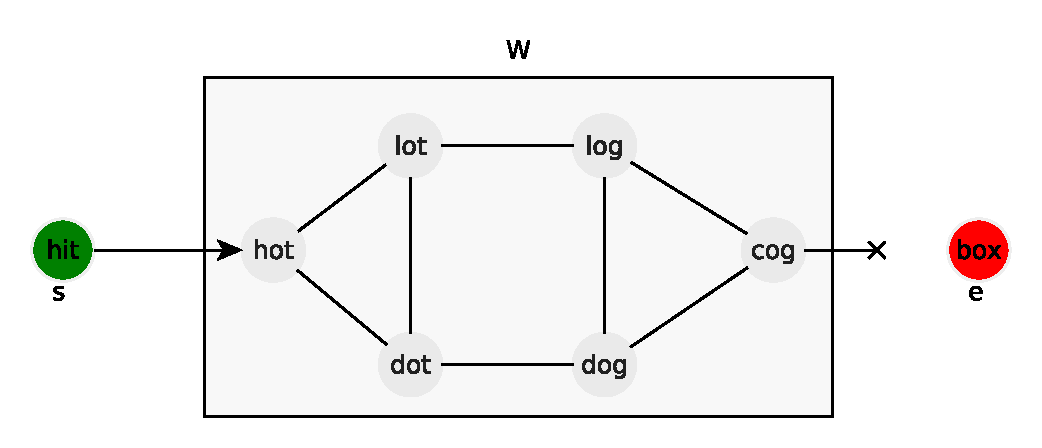
\includegraphics[width=\textwidth]{sources/word_ladder/images/example2}
        \caption[n]{Graph representation of Example \ref{example:word_ladder:example1} when $e=$\textit{box}. Notice how node \textit{box} is disconnected from the component containing \textit{hit}.}
        \label{fig:word_ladder:example1_impossible}
    \end{figure}
    

\lstinputlisting[language=c++, caption={Solution using BFS. Nodes different in exactly one character are connected.},label=list:word_ladder_bfs]{sources/word_ladder/word_ladder_solution1.cpp}

The code works by not explicitly constructing $G$ but instead by operating on an implicit graph. This implicit graph can be maintained by only keeping track of the visited nodes/words. 

\inline{word_ladder_BFS} is the main driver function and all it does is:
\begin{itemize}
    \item copying the elements of $W$ into an \inline{std::unordered_set} so that we can quickly check whether a string belongs to $W$ without having to perform a linear search.
    \item constructing a queue of \inline{std::pair<std:string, int>} as for each node/word we visit we want to remember its level (distance from $s$).
\end{itemize}.

The function \inline{addNeighbors} takes care of updating the BFS queue by generating all possible neighbors of a word $w$ having level \inline{count}. 
It does so by creating copies of $w$ that only differ in one position. If such a modified copy happens to be in $W$ then it is added to the queue with an incremented \inline{count} (signaling we need a step more to reach this new word from $w$).

The complexity of Listing \ref{list:word_ladder_bfs} is $O(|W|)$ for both time (albeit with a potentially high constant factor) and space.